\chapter{エクスパンダーグラフ概論} \label{chap:expander graph}
\section{定義}
グラフ$G=(V,E)$は, 単純ランダムウォークの非自明な第二固有値$\lambda(P)$が小さいときにエクスパンダーであるという.
多くの文脈では通常, 正則グラフに対してのみエクスパンダー性が定義されるが
本講義では一般のグラフに対してエクスパンダー性を定義する.
\begin{definition}{エクスパンダー}{expander}
    グラフ $G=(V,E)$上の単純ランダムウォークの遷移確率行列$P$が$\lambda(P) \le \lambda$を満たすときグラフ$G$は\emph{$\lambda$-エクスパンダー ($\lambda$-expander)}という.
    また, $P$の第二固有値が$\lambda_2 \le \lambda$を満たすとき, グラフ$G$は\emph{片側$\lambda$-エクスパンダー (one-sided $\lambda$-expander)}という.
\end{definition}
本講義ではエクスパンダー性を持つ単体複体も取り扱うため,
エクスパンダー性を持つグラフのことを\emph{エクスパンダーグラフ}と呼んで区別する.

要するにグラフのエクスパンダー性とは単純ランダムウォークの混交時間が小さいという性質を意味する.
二部グラフは周期的であり特に最小固有値が$\lambda_{|V|}=-1$となるためこの意味ではエクスパンダーグラフになりえないが,
片側エクスパンダーであるならば
遅延単純ランダムウォークの混交時間は小さくなる.

ランダムウォークの混交時間が小さいとはランダムウォークが「すぐに混ざり合う」ことを意味する.
この「すぐに混ざり合う」性質から, ランダムウォーク$(X_t)_{t\ge 0}$が時刻$t$までに訪れた頂点の集合を$U_t = \cbra*{X_0,\dots,X_t}$とすると, $\abs{U_t}$はすぐに拡大(expand)していく.

\paragraph*{例1 完全グラフ.}
グラフ$\rbra*{V, \binom{V}{2}}$を\emph{完全グラフ (complete graph)}という.
$n$頂点完全グラフ上の単純ランダムウォークの遷移確率行列$P$は, 単位行列$I$と全成分が$1$の行列$J$を用いて
$P = \frac{1}{n-1}(J-I)$で表せる.
完全グラフは正則グラフなので定常分布$\pi$は$V$上の一様分布である.
第一固有値は$\allone$であり,
その他の固有ベクトル$x_i$($i\ge 2$)は全て$\allone$に直交し, 特に$Jx_i = 0$となる.
従って$P x_i = -\frac{1}{n-1}x_i$なので, $\lambda_1=1$, $\lambda_2=\dots=\lambda_n = -\frac{1}{n}$である.
よって, $n$頂点完全グラフは$(1/n)$-expanderであると同時に片側$(-1/n)$-エクスパンダーグラフである
($\lambda(P)$の定義では絶対値をつけているが片側エクスパンダー性の定義では絶対値をつけていないことに注意).
%
\paragraph*{例2 閉路グラフ.}
頂点数$n$の閉路グラフとは, 頂点集合$V=\cbra{v_1,\dots,v_n}$に対して
辺集合$E$が$E = \cbra{\cbra{v_1,v_2},\dots,\cbra{v_{n-1},v_n}, \cbra{v_n,v_1}}$で与えられるグラフ$(V,E)$である.
頂点数$n$が偶数のとき, 閉路グラフは二部グラフとなる.

ここでは$\omega = \exp\rbra*{\frac{2\pi \mathrm{i}}{n}}$を$1$の冪根とし,
頂点集合を$V=\cbra{\omega^i \colon i=0,\dots,n-1}$とし, 各辺を$\cbra{\omega^i,\omega^{i+1}}$で表す.
任意の関数$f\colon V\to \Real$に$P$を作用させると
\[ Pf(\omega^i) = \frac{f(\omega^{i-1}) + f(\omega^{i+1})}{2}\]
を得る.
関数$x_k\colon \omega^j \mapsto \omega^{kj}$を考えると,
$Px_k (\omega_j) = \frac{\omega^{k(j-1)} + \omega^{k(j+1)}}{2} = \frac{\omega^{-k}+\omega^{-k}}{2}\cdot x_k(\omega_j)$を得る.
従って各$k=0,\dots,n-1$に対し$x_k$はそれぞれ固有値$\frac{\omega^k + \omega^{-k}}{2} = \cos\frac{2\pi k}{n}$に対応する固有ベクトルである.

これらの固有値を降順に並べて$1=\lambda_1\ge \dots\ge \lambda_n\ge-1$とすると,
$\lambda_2 = \cos\frac{2\pi}{n} = 1-\frac{4\pi^2}{2n^2} + O(n^{-4})$である.
頂点数$n$が偶数のときは$\lambda_n = -1$,
頂点数$n$が奇数のときは$\lambda_n = \cos\pi\rbra*{1 - \frac{1}{n}} = -\cos\frac{\pi}{n} = -1 + \frac{\pi^2}{2n^2} - O(n^{-4})$である.
従って頂点数$n$が奇数のときの閉路グラフは$\cos\frac{\pi}{n}$-エクスパンダーであり,
$n\to\infty$の漸近を考えると$n$のスペクトルギャップは$\Theta(1/n^2)$となる.

\section{存在性と陽な構成}
エクスパンダー性はランダムウォークがすぐに混ざり合うということを意味し, これを満たすグラフは多くの辺を持つべきである.
例えば完全グラフは非常に強いエクスパンダー性を持つ一方で閉路グラフのエクスパンダー性は乏しい.
では, 疎でありかつエクスパンダー性をもつグラフは存在するだろうか?
また, 陽に構成できるだろうか?
%
\subsection{Margulisの構成}
定数$\lambda<1$に対し$\lambda$-エクスパンダーの族は\citet{Margulis1973}によって初めて与えられ,
そのスペクトルギャップの陽な値は\citet{GG81}により初めて与えられた.
より詳細な背景や定理の証明は\cite{HLW06}を参照されたい.
\begin{theorem}{Margulisの構成}{Margulis construction}
    グラフ族$(G_m)_{m\in\Nat}$を以下で定義する:
    頂点集合$V_m$は$V_m=\mathbb{Z}_m \times \mathbb{Z}_m$とし,
    \begin{align*}
        T_1 = \begin{bmatrix}
            1 & 2 \\
            0 & 1
        \end{bmatrix},& &
        T_2 = \begin{bmatrix}
            1 & 0 \\
            2 & 1
        \end{bmatrix},& &
        e_1 = \begin{bmatrix}
            1 \\
            0
        \end{bmatrix}, & &
        e_2 = \begin{bmatrix}
            0 \\
            1
        \end{bmatrix}
    \end{align*}
    とする.
    各頂点$v=(x,y)\in V_m$を$T_1v,T_2v,T_1v+e_1,T_2v+e_2$およびこれらの逆変換で与えられる八つの頂点と接続させて得られるグラフを$G_m$とする (多重辺や自己ループも含みうる).

    このとき, 任意の$m\in\Nat$に対して$\lambda(G_m) \le \frac{5\sqrt{2}}{8} < 0.9$.
\end{theorem}

\subsection{ケイリーグラフ}
エクスパンダーグラフを陽に構成する最も重要なアプローチの一つとして
ケイリーグラフ\cite{Cayley1878}と呼ばれる概念が知られている.

%
\begin{definition}{ケイリーグラフ}{Cayley graph}
    $G$を有限群, $A\subseteq G$を$G$の生成系\footnote{任意の$g\in G$に対してある有限個の$a_1,\dots,a_m\in A$を用いて$g=\prod_{i=1}^ma_i$と表せるとき, $A\subseteq G$は生成系であるという.}であって単位元を含まず, 逆元で閉じている(i.e., $A^{-1}=\{a^{-1}\colon a\in A\}=A$)ものとする.
    頂点集合$V=G$, 辺集合$E=\{\{g,ag\}\colon g\in G,a\in A\}$に対し$(V,E)$で与えられるグラフを\textbf{ケイリーグラフ(Cayley graph)}といい, $\Cay(A,G)$で表す.
    頂点$g\in G$に対し, $E_g=\{\{g,ag\}\colon a\in A\}$を$g$を含む辺の集合とする.
\end{definition}
%
ケイリーグラフは群の幾何学的な性質を調べる幾何学的群論における重要な研究対象の一つである.
$A$は単位元を含まないため自己ループは存在しない.
また, $A^{-1}=A$より$\{ag,a^{-1}(ag)\}\in E$となるため$\Cay(A,G)$は無向グラフとなっている.
同様にケイリーグラフ$\Cay(G,A)$も考えることができるが, 写像$x\mapsto x^{-1}$を考えると$\Cay(A,G)$と$\Cay(G,A)$が同型になっているので本質的には同じである.
ケイリーグラフ$\Cay(A,G)$は$|A|$-正則グラフである.


\subsection{Alon-Boppanaの定理}
グラフの辺数を固定したとき, エクスパンダー性のパラメータ$\lambda$はどこまで小さくできるだろうか?
ここでは厳密な証明は与えずに直感的な議論によって正則グラフに絞ってエクスパンダー性の限界を説明する.

あとの節(\cref{sec:expander graph application})で詳しく述べるが,
応用上は正則なエクスパンダーグラフが重要である.
正則グラフ上のランダムウォークの遷移確率行列は単に隣接行列を次数で割ったものであり定常分布も一様分布なので
単に隣接行列の固有値を考えれば良いことがわかる.\footnote{これらの理由からエクスパンダーグラフの理論は多くの教科書では正則グラフ上でのみ展開されている.}

固定した自然数$d\ge 3$に対して最もエクスパンダー性の強い(つまり$\lambda$が最小となる)$d$-正則グラフはどのようなグラフだろうか?
問題を言い換えればランダムウォークがより多くの頂点を訪れやすくするにはグラフをどのように構成すれば良いだろうか?

直感的な議論だが, 短い閉路があるとそれに沿って同じ頂点を訪れてしまうので, そのような閉路はない方が良いと思われる.
従ってそのグラフを虫眼鏡でズームすると局所的には木構造になっているべきであろう.
そこで「理想的な」グラフとして$d$-正則で頂点数が無限の木$T$を考える.
頂点集合$V$は可算無限であるため, 有限グラフに対する隣接行列や固有値の概念を無限グラフに拡張したものが必要である.
集合$\ell^2(V) \subseteq \Real^V$を
$\ell^2(V) = \cbra*{ f \colon V \to \Real\colon \sum_{u\in V}f(u)^2 < \infty }$とする.
隣接作用素$A\colon \ell^2(V) \to \ell^2(V)$を
\[
    A f(u) = \sum_{v \in N_T(u)} f(v)
\]
で定める.
ここで$N_T(u)\subseteq V$は$T$において$u$と隣接している頂点の集合であり, $T$の$d$-正則性から
有限集合である.
このように$\ell^2(V)$上の作用素とすることによって, 非ゼロの定数関数を自然に除外しているのである!
作用素$A$のスペクトルを
\[
    \mathrm{spec}(A) = \cbra*{ \lambda \in \Real \colon A - \lambda I\text{ は退化}}
\]
とする.
\begin{theorem}{}{infinite d-regular tree spectral}
    $d$-正則無限木$T$の隣接作用素$A$のスペクトルは以下を満たす:
    \[ \mathrm{spec}(A) \subseteq [-2\sqrt{d-1}, 2\sqrt{d-1}].\]
\end{theorem}
従って, 理想的なグラフを考えるとその隣接行列の非自明な固有値はその絶対値が高々$2\sqrt{d-1}$である
(第一固有ベクトル$\allone$に対応する関数は$\ell^2(V)$に属さない).
よって任意の$d$-正則グラフは$\lambda(P)\ge \frac{2\sqrt{d-1}}{d}$を満たすであろうことが予想される.

\subsection{Alon-Boppanaの定理}
定数次数の正則グラフの直径は$\Omega(\log n)$を満たす.
\begin{lemma}{}{regular graph diameter}
    $d\ge 3$のとき,
    $n$頂点$d$-正則連結グラフ$G=(V,E)$の直径は$\diam(G) \ge \log_{d-1}\frac{(d-2)(n-1)}{d}$を満たす.
\end{lemma}
\begin{proof}
    頂点$u\in V$を固定すると, $u$から$\ell$本以下の辺を辿って辿り着ける頂点は高々
    \[ 1 + d + d(d-1) + \dots + d(d-1)^{\ell-1} \le 1 + d(d-1)^{\ell-1}\sum_{i=0}^{\ell-1}\rbra*{\frac{1}{d-1}}^i \le 1+\frac{d(d-1)^\ell}{d-2}  \]
    この最右辺が$n$より真に小さいとき, $u$から$\ell$本以下の辺を辿って辿り着けない頂点が存在する.
    従って, $\ell=\diam(G)$を代入したときの最右辺は$n$以上でなければならないため,
    不等式$1+\frac{d(d-1)^{\diam(G)}}{d-2}\ge n$を解くと主張を得る.
\end{proof}

\begin{theorem}{Alon--Boppanaの定理}{Alon Boppana}
    ある定数$c>0$が存在し, 任意の$n$頂点$d$正則グラフ$G$上の単純ランダムウォークの遷移確率行列$P$の第二固有値$\lambda_2$は
    \[ \lambda_2 \ge \frac{2\sqrt{d-1}}{d}\rbra*{ 1 - \frac{c}{\diam(G)^2}} \]
    を満たす.
\end{theorem}
特に, \cref{lem:regular graph diameter}より, 次数$d\ge 3$を固定して頂点数$n\to\infty$の漸近において$\ell = \Omega(\log n)$であるため, $\lambda_2 \ge \frac{2\sqrt{d-1}}{d} (1 - O(1/\log^2 n))$を満たす.
この結果は次数$d$を固定したときの正則グラフのエクスパンダー性のパラメータの限界を表している.

ここでは少し弱い下界として
\begin{align}
    \lambda_2 \ge \frac{2\sqrt{d-1}}{d}\rbra*{1 - O\rbra*{\frac{\log \diam(G)}{\diam(G)}}} \label{eq:weak alon boppana bound}
\end{align}
を証明する. この下界でも$\lambda_2 \ge \frac{2\sqrt{d-1}}{d}(1-o(1))$を示すには十分である.
\begin{proof}[\textbf{\cref{eq:weak alon boppana bound}の証明.}]
    遷移確率行列を$P$とし, 隣接行列を$A$とする.
    二頂点$u,v$を$uv$間の最短路が$\diam(G)$に等しくなるように固定し
    関数$f \colon V \to \Real$を$f = \delta_s - \delta_t$とすると, 任意の$k\ge 1$に対して
    \begin{align*}
        \lambda(P^{2k}) & = \lambda(P^k)^2                                                                                                \\
                        & \ge \frac{\piprod{f,P^{2k} f}}{\pinorm{f}^2}                  &  & \text{$\because$\cref{lem:Rayleigh quotient}} \\
                        & = \frac{P^{2k}(u,u) + P^{2k}(v,v) - 2P^{2k}(u,v)}{2}                                                            \\
                        & = \frac{A^{2k}(u,u) + A^{2k}(v,v) - 2A^{2k}(u,v)}{2d^{2k}}. &  & \text{$\because P=\frac{1}{d}A$}
    \end{align*}
    \cref{lem:adjacency walk count}より, $k=\floor*{\frac{\diam(G)-1}{2}}$とすると, $u,v$の選び方より$A^{2k}(u,v)=0$である.
    \cref{lem:adjacency walk count}より, $A^{2k}(u,u)$は頂点$u$を含む長さ$2k$の閉路の個数に等しい.
    さらに, この値は$d$-正則無限木$T$において固定した頂点を含む長さ$2k$の閉路の個数で下から抑えることができる.

    \begin{lemma}{正則グラフの閉路数の下界}{closed walk regular graph}
        $d\ge 3$に対し, $T$を$d$-正則無限木とし, 頂点を一つ固定する.
        この頂点を含む長さ$2k$の閉路の個数を$t_{2k}$とすると
        \[ t_{2k} \ge (d-1)^{k}\cdot \frac{1}{k+1}\binom{2k}{k} \]
        である.
        さらに,
        任意の$d$-正則グラフ$G=(V,E)$の任意の頂点$u$に対し, $u$を含む長さ$2k$の閉路の個数は少なくとも$t_{2k}$である.
    \end{lemma}

    まずは\cref{lem:closed walk regular graph}を認めて\cref{thm:Alon Boppana}の証明を完成させる (\cref{lem:closed walk regular graph}は後で証明する).
    二項係数$\binom{2k}{k}$はStirlingの近似により$\binom{2k}{k} \ge \frac{4^k}{\sqrt{\pi k}}\rbra*{1-\frac{1}{8k}}$を満たすことが示せる.
    従って, \cref{lem:closed walk regular graph}より,
    \begin{align*}
        \lambda(P)^{2k} & \ge d^{-2k} t_{2k}                                                                     \\
                        & \ge d^{-2k}\cdot (d-1)^k \cdot \frac{2^{2k}}{(k+1)\sqrt{\pi k}}\rbra*{1-\frac{1}{8k}}.
    \end{align*}
    特に, ある定数$c>0$が存在して
    \begin{align*}
        \lambda(P) & \ge \frac{2\sqrt{d-1}}{d} \cdot k^{-c/k}                            \\
                   & \ge \frac{2\sqrt{d-1}}{d}\cdot \rbra*{1-O\rbra*{\frac{\log k}{k}}}.
    \end{align*}
    最後の不等号は$k^{-k}=\e^{-\frac{\log k}{k}} = 1-O\rbra*{\frac{\log k}{k}}$を用いた.
    $k=\floor*{\frac{\diam(G)-1}{2}}$を代入すれば\cref{eq:weak alon boppana bound}を得る.
\end{proof}
最後に\cref{lem:closed walk regular graph}を証明する.
\begin{proof}[\textbf{\cref{lem:closed walk regular graph}の証明.}]
    $d$-正則無限木$T$の特別な頂点$v_0$を一つ固定し, (グラフ理論においてスタンダードな)幾つかの用語を定義する.
    固定した特別な頂点$v_0$を\emph{根 (root)}と呼び,
    $T$の頂点$v$に対し, $\dist(v_0,v)$を\emph{深さ (depth)}と呼び$\mathrm{depth}(v)$で表す (特に$\mathrm{depth}(v_0)=0$である).
    頂点$v$に$T$上で隣接している$d$個の頂点からなる集合を$N_T(v)$と表す ($N_T(v)$に$v$は含めない).
    これらの隣接頂点のうち, 深さが$\mathrm{depth}(v)-1$となるただ一つの頂点を$v$の\emph{親 (parent)}と呼び,
    残りの深さ$\mathrm{depth}(v)+1$の頂点を$v$の\emph{子 (child)}と呼ぶ.

    \begin{figure}
        \begin{center}
            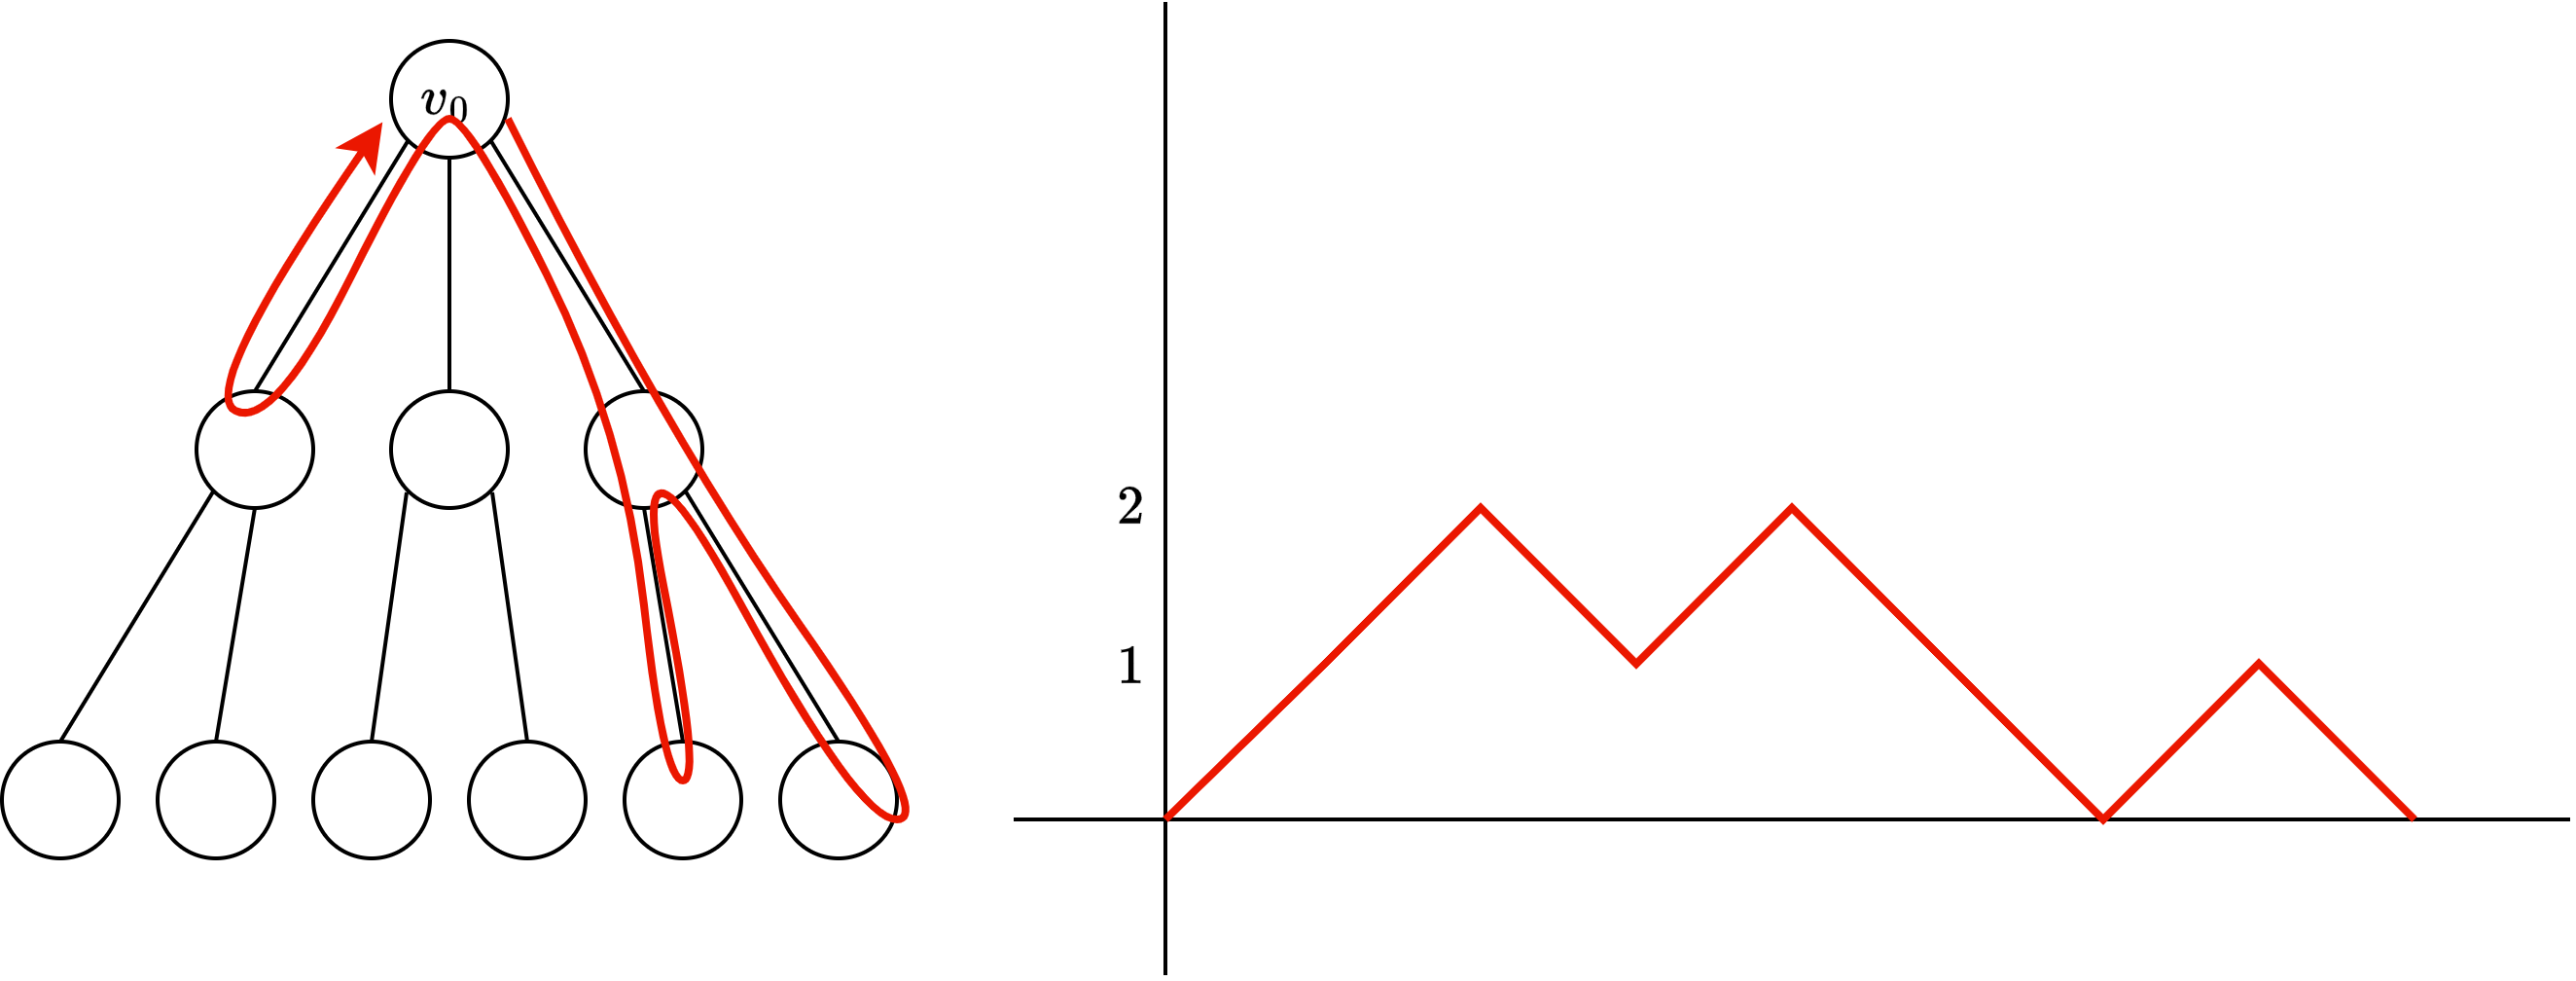
\includegraphics[width=12cm]{images/tree.png}
            \caption{$3$正則木$T$上の長さ$10$の閉路. 親から子への遷移と子から親への遷移を$5$回ずつ行う. 右図は深さ$d_i$の遷移を表す.}
        \end{center}
    \end{figure}

    木$T$において根を始点とする長さ$2k$の閉路$(v_0,\dots,v_{2k})$を考える (ここで$v_0=v_{2k}$).
    各$i$に対して$d_i = \mathrm{depth}(v_i)$とし, 列$(d_0,\dots,d_{2k})$を考える.
    まず$d_0=0$であり, その後は$d_{i+1} \in \cbra{d_i \pm 1}$であり, 常に非負を保ちながら最後に$d_{2k}=0$となる.
    このような列$(d_0,\dots,d_{2k})$の総数はカタラン数と等しく, $\frac{1}{k+1}\binom{2k}{k}$に等しい.
    特に, 各$d_i - d_{i-1}$の符号を見ると$d_0 = d_{2k} = 0$より正と負がそれぞれ$k$個ずつ含まれている.

    次に, 各$(d_1,\dots,d_{2k})$に対して深さの履歴がこれと等しくなるような閉路の個数を考える.
    各$i\ge 2$において, $d_i=d_{i-1}+1$ (すなわち$v_i$が$v_{i-1}$の子である)とき, $v_i$の選び方は少なくとも$d-1$通りある ($v_i$が根であるときは$d$通りあるがこれも下から$d-1$で抑える).
    一方で親に遷移する場合はその遷移先は一意である.
    子への遷移はちょうど$k$回発生するため, 深さの履歴が与えられた$(d_1,\dots,d_{2k})$に等しくなるような閉路の個数は少なくとも$(d-1)^{k}$個存在する.
    従って$t_{2k} = \frac{1}{k+1}\binom{2k}{k} \cdot (d-1)^{k}$を得る.

    後半の主張を証明する.
    $d$-正則グラフ$G$の頂点$u_0$を一つ固定する.
    木$T$の頂点集合を$U$, グラフ$G$の頂点集合を$V$とし,
    $N_T$の定義と同様にグラフ$G$の頂点$v \in V$に対しその$d$個の隣接頂点の集合を$N_G(v)$で表す.
    $G$から$T$への準同型写像$\phi \colon U \to V$を以下のように構成する\footnote{グラフ$G=(V,E)$から$H=(W,F)$への\emph{準同型写像 (homomorphism)}とは, 写像$\phi\colon V\to W$であって$\{u,v\}\in E\Rightarrow \{\phi(u),\phi(v)\}\in F$を満たすものである. ここでは自然に無限グラフに対してこの概念を拡張している.}:
    深さに関して帰納的に定義する.
    \begin{itemize}
        \item まず, $\phi(v_0) = u_0$とする.
              根$v_0$の子$N_T(v_0)$から$N_G(u_0)$への全単射$\phi_0$を任意に一つ選び,
              $\phi\colon N_T(v_0) \ni v' \mapsto \phi_1(v') \in N_T(u_0)$
              によって$N_T(v_0)$における$\phi$を定義する.
        \item $T$における深さ$\ell$以下の全ての頂点に対し$\phi(v)$が定義されているとする. 深さ$\ell$の各頂点$v$に対し, その親を$p$, 子を$c_1,\dots,c_{d-1}$とする. $v$とその親$p$に対しては$u\defeq \phi(v)$, $u_p\defeq \phi(p)\in U$が定義されている. このとき, 全単射$\psi\colon N_T(v)\setminus \{p\} \to N_G(u)\setminus\{u_p\}$を任意に一つ固定し, 各$\phi(c_j)$を$\psi(c_j)\in V$とする.
    \end{itemize}
    このようにして定義された写像$\phi\colon U \to V$は確かに準同型なので
    $T$の閉路$(v_0,\dots,v_{2k})$に対して$(\phi(v_0),\dots,\phi(v_{2k}))$は$G$の閉路になっている.
    さらに, $(\phi(v_0),\dots,\phi(v_{2k}))$の形になっている$G$の閉路が与えられたとき, $v_0$は一意に定まり, 以降の$v_i$は$\phi$の帰納的な定義で用いた全単射の逆写像を用いて順番に復元することができるため, $(v_0,\dots,v_{2k}) \mapsto (\phi(v_0),\dots,\phi(v_{2k}))$は単射である.
    従ってグラフ$G$に含まれるある頂点を始点とした長さ$2k$の閉路の個数は少なくとも$t_{2k}$である.
\end{proof}


\subsection{ラマヌジャングラフ}
漸近的に\cref{thm:Alon Boppana}を達成するグラフを\emph{ラマヌジャングラフ (Ramanujan graph)}という.
\begin{definition}{ラマヌジャングラフ}{Ramanujan graph}
    $d$-正則グラフ$G=(V,E)$は, その単純ランダムウォークの遷移確率行列$P$の第二固有値$\lambda_2$が$\lambda_2 \le 2\sqrt{d-1}$を満たすとき, \emph{ラマヌジャングラフ (Ramanujan graph)}という.
\end{definition}

\cref{thm:Alon Boppana}を達成するグラフ列, すなわち,
次数$d$を固定したときに頂点数が増大していくグラフ列$(G_n)_{n\in\Nat}$であって各$G_n$が$d$-正則ラマヌジャングラフとなるものは存在
するだろうか?
この漸近的に最適な正則エクスパンダーグラフの構成は\citet{LPS88,Mar88}によって独立同時期に初めてその構成が与えられた.
彼らは$d-1$が$4$で割った余りが$1$となる素数であるときに$d$-正則ラマヌジャングラフの列を構成した.
なお, 「ラマヌジャングラフ」という名称は\cite{LPS88}の証明がラマヌジャン予想と呼ばれる予想に依拠しているからである
(「予想」と書いたが当時は既に解決している).
その後, \citet{Mor94}によって次数が素数べき$+1$の形であってもラマヌジャングラフが構成できることが示された.
\begin{theorem}{ラマヌジャングラフの陽な構成}{LPS Ramanujan}
    任意の素数$q$と任意の$k\in\Nat$に対して, 頂点数が発散するある$(q^k+1)$-正則ラマヌジャングラフの列が存在し, 陽に構成できる.
\end{theorem}
%また, \cite{LPS88}とは独立同時期に\citet{Mar88}もラマヌジャングラフの族を構成しているようである
%    (元論文はロシア語で書かれており, 英語に翻訳されたものもあるようなのだが見つけることはできなかった).

\paragraph*{ランダム正則グラフ.}
\citet{LPS88}やその後続研究によりラマヌジャングラフ列については様々な構成方法が知られている.
では, そもそもラマヌジャングラフは何個あるのだろうか?
$n$頂点$d$-正則グラフ全体の集合を$\calG_{n,d}$とし,
$\calG_{n,d}$から一様ランダムに選ばれたグラフ$G\sim\calG_{n,d}$を考える
($nd$は常に偶数とする).
この確率変数をランダム正則グラフという.
ランダム正則グラフは「ほぼ」ラマヌジャングラフであることが知られている
\cite{Friedman_random_regular}.
\begin{theorem}{Friedmanの定理}{random regular graph Ramanujan}
    任意の$d\ge 3$と任意の$\varepsilon > 0$に対し,
    \[ \lim_{n\to\infty}\Pr\sbra*{\lambda(P) \ge \frac{2\sqrt{d-1}}{d} + \varepsilon} = 0. \]
\end{theorem}
すなわち, ほとんど全ての定数次数正則グラフはラマヌジャングラフとほぼ同等のスペクトルを持つ.

\subsection{ジグザグ積による組合せ的な構成}
\begin{definition}{置換積}{replacement product}
    グラフ$G=(V,E)$を$N$頂点$D$-正則グラフとし, グラフ$H=([D],F)$を$[D]$を頂点集合に持つ$D$頂点$d$-正則グラフとする.
    グラフ$G$の各頂点$u\in V$の隣接頂点は$1$から$D$の番号づけが付随していて$N(u)=\{u_1,\dots,u_D\}$とする.

\end{definition}

\section{性質}
エクスパンダーグラフは固有値によって定義されるが, 様々な興味深い性質を持つことが知られている.
ここではグラフ理論的な性質と擬似ランダム性について紹介する.
%


\subsection{擬似ランダム性(*)} \label{sec:expander pseudorandom}
この節は高次元エクスパンダーの本筋から少し外れるが,
エクスパンダーグラフの重要であることの理由の一つとしてその擬似ランダム性について概説する.

加法的組合せ論や計算量理論では\emph{擬似ランダム性 (pseudorandomness)}と呼ばれる概念が非常に重要な役割を果たしている.
\begin{definition}{分布の擬似ランダム性}{pseudorandomness}
    有限集合$\Omega$上のある分布$\mu$と関数族$\mathcal{F} \subseteq \{f\colon \Omega \to \binset\}$を考える.
    分布$\mu$は,
    任意の$f\in \mathcal{F}$に対して
    \[ \abs*{\E_{x\sim \mu} [f(x)] - \E_{y\sim U_{\Omega}}[f(y)]} \le \varepsilon\]
    を満たすとき, \emph{$\mathcal{F}$に対して$\varepsilon$-擬似ランダムである}という (ここで, $y\sim U_\Omega$とは$\Omega$上一様ランダムに$y$が選ばれたことを意味する).
\end{definition}
直感的には, 分布が擬似ランダムであるとは, その分布が任意の$f\in \mathcal{F}$を使っても一様分布と\emph{識別できない (indistinguishable)}ことを意味する.
例えば全変動距離に関する\cref{prop:dtv}では, $\mathcal{F}$を$V$上の二値関数全体 (すなわち任意の$V$の部分集合)の族としたときの識別不可能性のパラメータ$\varepsilon$が全変動距離で与えられることを意味する.
すなわち$\mu$は常に$\dtv(\mu,U_{\Omega}))$-擬似ランダムである.
関数クラス$\mathcal{F}$をより制限したときにパラメータ$\varepsilon$がどこまで小さくなるかに興味がある.

組合せ論では$\mathcal{F}$としてある特殊な関数クラスを仮定することによって\emph{組合せ論的擬似ランダム性}を定義する.
例えばグラフ理論や加法的組合せ論のコーナーストーンの一つと呼ばれるSzemerédiの正則化補題と呼ばれる結果は, 非常に大雑把に言えば
任意の密なグラフが定数個の擬似ランダムな二部グラフと疎な部分に分解できることを主張する定理である.
組合せ論的擬似ランダムネスの概念は特に加法的組合せ論において非常な協力な道具となっており,
Green--Taoの定理の証明においても重要な役割を果たしている
(驚くべきことに, 識別不可能性の枠組みでGreen--Taoの定理の証明を理解してそれを学習理論におけるブースティングの証明に応用するという研究もなされている!).

計算量理論では$\mathcal{F}$を「効率的なアルゴリズムの全体」や「素子数の少ない論理回路の全体」とすることで\emph{計算量的擬似ランダム性}を定義できる.
任意の効率的なアルゴリズムに対して一様ランダムな文字列と識別できないということは, その分布に従って生成されたメッセージを盗み見てもそこから得られる情報が何もない (ランダムな文字列を見てるのと同じ) であることから, 計算量的擬似ランダム性は暗号の計算量的安全性の定義の根幹をなすことがわかる.

エクスパンダーグラフの組合せ論的擬似ランダム性を説明する.
正則$\lambda$-エクスパンダー$G=(V,E)$を考える.
集合$\Omega=V\times V$上の分布$\mu = \mu_G$として
一様ランダムな辺$\{u,v\}\in E$を選び, $(u,v)$もしくは$(v,u)$どちらかを等確率で選んだ時の頂点対の分布とする.
すなわち,
\begin{align}
    \Pr_{(u,v)\sim \mu}\sbra*{ (u,v) = (s,t)} = \frac{\indicator{\{s,t\}\in E}}{2\abs{E}} = \frac{\indicator{\{s,t\}\in E}}{nd} \label{eq:expander mu}
\end{align}
とする.
関数族$\mathcal{F}$を
\begin{align}
    \mathcal{F} = \cbra*{ f_{S,T} \colon (s,t) \mapsto \indicator{s\in S,t\in T} \colon S,T\subseteq V}  \label{eq:expander F}
\end{align}
で定める.

以下の結果は\citet{AC88}によるものである.
%
\begin{lemma}{エクスパンダー混交補題}{expander mixing lemma}
    任意の頂点部分集合$S,T\subseteq V$に対して,
    $e(S,T) = \sum_{s\in S,t\in T} \indicator{\{s,t\} \in E}$を$S,T$間の辺の本数($S\cap T$内の辺は2回数える)とすると,
    \[
        \abs*{e(S,T) - \frac{d}{n}|S||T|} \le d\lambda\sqrt{|S||T|\rbra*{1-\frac{|S|}{n}}\rbra*{1-\frac{|T|}{n}}}.
    \]
    同様に, $G$が片側$\lambda$-エクスパンダーならば,
    \[
        e(S,T) - \frac{d}{n}|S||T| \le d\lambda\sqrt{|S||T|\rbra*{1-\frac{|S|}{n}}\rbra*{1-\frac{|T|}{n}}}.
    \]
\end{lemma}

\begin{corollary}{擬似ランダム性}{pseudorandomness expander}
    グラフ$G$が$n$頂点$d$-正則$\lambda$-エクスパンダーであるとき, \cref{eq:expander mu}で定義された分布$\mu$は\cref{eq:expander F}で定義された関数族$\mathcal{F}$に関して$\frac{\lambda}{4}$-擬似ランダムである.
\end{corollary}
%
グラフ$G$の隣接行列$A$を考えるとイメージしやすい.
この行列は全部で$nd$個の$1$を持っているため, 全成分の中で$1$の密度は$\frac{d}{n}$である.
ここで, 部分集合$S,T\subseteq V$に対して$A$の$S\times T$で定まる部分行列$A_{S,T}$を考える.
この行列に含まれる$1$の個数($e(S,T)$に等しい)は, $\frac{d}{n}\cdot |S||T|$に近い値となっている (\cref{fig:EML}).
\begin{figure}[htbp]
    \begin{center}
        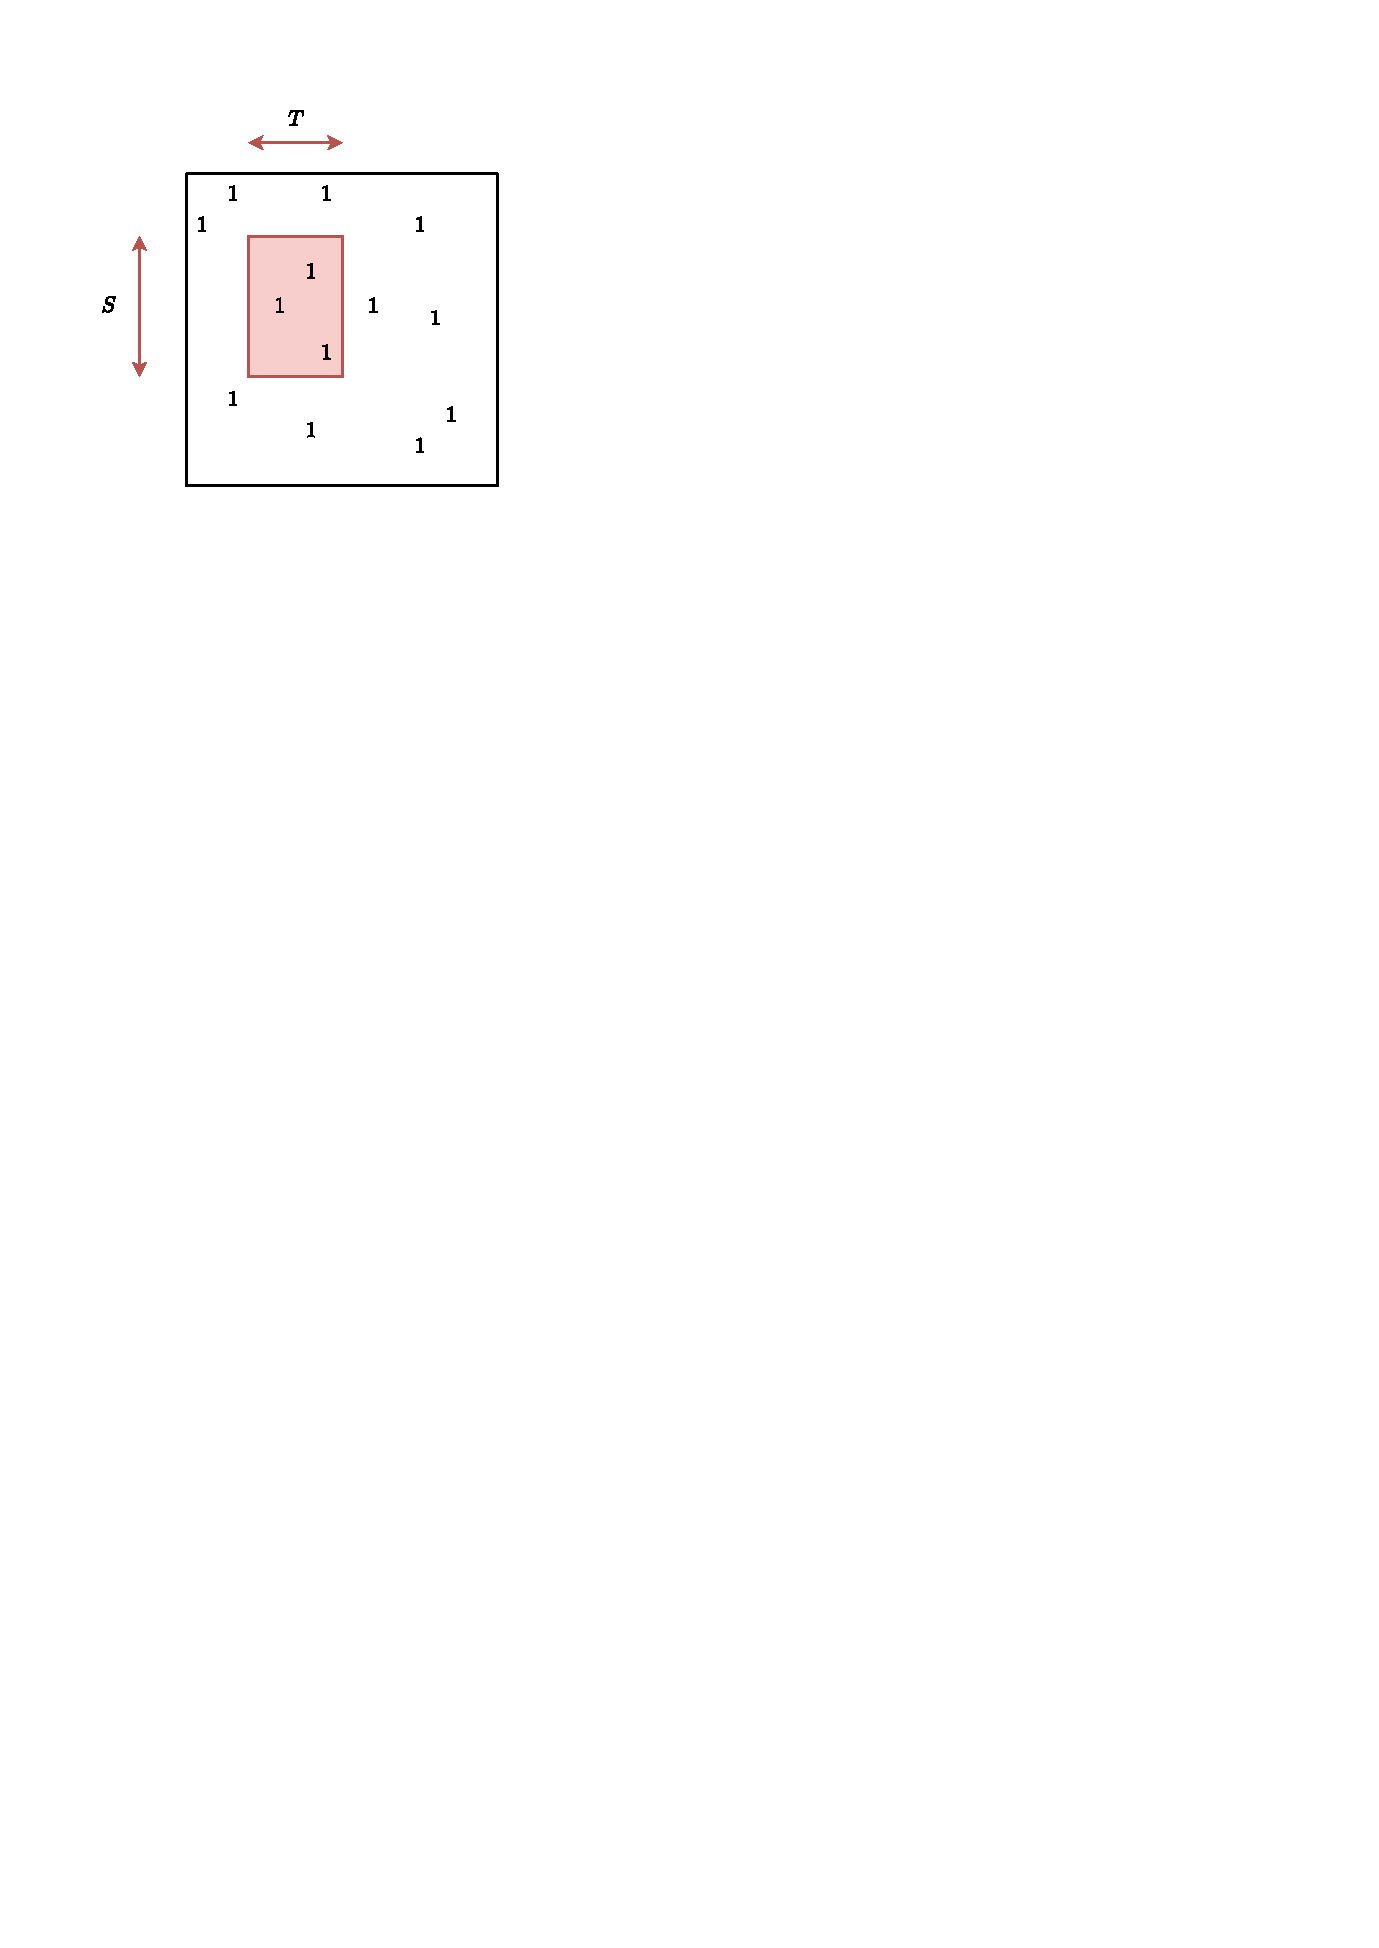
\includegraphics[width=6cm]{images/EML.pdf}
        \caption{正則グラフの隣接行列$A$を考える. このグラフがエクスパンダーならば, 頂点部分集合$S,T\subseteq V$で指定される長方形内に含まれる$1$の密度は行列全体の$1$の密度に近い値をとる. \label{fig:EML}}
    \end{center}
\end{figure}
%
\begin{proof}[\cref{lem:expander mixing lemma}の証明.]
    グラフ$G$上の単純ランダムウォーク$P$を考える.
    部分集合$S,T\subseteq V$に対し
    関数$f=\delta_S,g=\delta_T$として
    \cref{cor:general expander mixing lemma}を適用すると
    \begin{align*}
         & \piprod{f,Pg} = \frac{e(S,T)}{nd},               \\
         & \Epi f = \frac{|S|}{n},                          \\
         & \Epi [Pg] = \Epi g = \frac{|T|}{n},              \\
         & \Varpi f = \frac{|S|}{n}\rbra*{1-\frac{|S|}{n}}, \\
         & \Varpi g = \frac{|T|}{n}\rbra*{1-\frac{|T|}{n}}
    \end{align*}
    より整理すると主張を得る.

    グラフ$G$が片側エクスパンダーである場合は\cref{cor:general expander mixing lemma}の代わりに\cref{lem:one side EML}を適用すればよい.
\end{proof}
\begin{exercise}{}{check}
    \cref{lem:expander mixing lemma}の証明で表した五つの等式を実際に確認せよ.
\end{exercise}
「エクスパンダー混交補題」と言うと聞こえが良いが, \cref{cor:general expander mixing lemma}を見るとその実は単なるCauchy--Schwarzの不等式とレイリー商の議論を適用しただけであることがわかる.

エクスパンダー混交補題の応用として, エクスパンダーグラフ上のランダムウォークはずっと同じ頂点部分集合にとどまらないことを示せる.
\begin{proposition}{}{expander walk hitting}
    グラフ$G=(V,E)$を$n$頂点$d$-正則片側$\lambda$-エクスパンダーとし,
    $(X_t)_{t\ge 0}$を$G$上の単純ランダムウォークで初期頂点$X_0$が$V$上一様ランダムに選ばれたものとする.
    任意の$\ell\in\Nat$と頂点部分集合$B\subseteq V$に対し, $\mu = \frac{|B|}{n}$とすると, 以下が成り立つ:
    \[
        \Pr\sbra*{\text{全ての$t=0,\dots,\ell$に対し}X_t \in B} \le \rbra*{ \mu + \lambda(1-\mu)}^\ell.
    \]
\end{proposition}
\begin{proof}
    $\ell\ge 0$に対し$\mathcal{E}_\ell$を「全ての$t=0,\dots,\ell$に対し$X_t\in B$」という事象とする.
    初期頂点$X_0$が定常分布($=$一様分布)に従って選ばれているため, 各$t$に対し$X_t$の周辺分布もまた一様分布である.
    特に, \cref{lem:expander mixing lemma}より, 任意の$t\ge 0$に対し
    \begin{align}
        \Pr\sbra*{ X_{t+1} \in B \text{ かつ }X_t \in B} &= \frac{e(B,B)}{nd} \nonumber\\
        &\le \mu^2 + \lambda\mu(1-\mu) \label{eq:eml bound}
    \end{align}
    を得る.
    従って
    \begin{align*}
        \Pr\sbra*{\mathcal{E}_\ell} &= \Pr\sbra*{ X_\ell \in B \condition \mathcal{E}_{\ell-1} }\cdot \Pr\sbra*{\mathcal{E}_{\ell-1}} \\
        &= \Pr\sbra*{X_\ell \in B \condition X_{\ell-1} \in B}\cdot \Pr\sbra*{\mathcal{E}_{\ell-1}} \\
        &= \frac{\Pr\sbra*{ X_{t+1} \in B \text{ かつ }X_t \in B}}{\mu} \cdot \Pr\sbra*{\mathcal{E}_{\ell-1}} \\
        &\le \rbra*{\mu + \lambda(1-\mu)}\cdot \Pr\sbra*{\mathcal{E}_{\ell-1}} & & \text{$\because$\cref{eq:eml bound}} \\
        &\dots \\
        &\le \rbra*{\mu + \lambda(1-\mu)}^\ell\cdot \Pr[\mathcal{E}_0] \\
        &\le \rbra*{\mu + \lambda(1-\mu)}^\ell
    \end{align*}
    より主張を得る.
\end{proof}

\subsection{グラフ理論的な性質}
本講義とは直接の関係はないが,
エクスパンダーグラフはグラフ理論的に非常に興味深い多くの性質を有するため,
いくつかを簡単に紹介する.
本節では主に正則グラフに対する組合せ論的な性質について述べる.

\begin{proposition}{低直径性}{small diameter}
    $n$頂点$(1-\gamma)$-エクスパンダーの直径は高々$\ceil*{\frac{12\log n}{\gamma}}$.
\end{proposition}
\begin{proof}
    二頂点$u,v$を任意に固定し,
    $u$を始点とした単純ランダムウォーク$(X_t)_{t\ge 0}$を考える.
    定常分布$\pi$は$\pimin \ge \frac{1}{2|E|} \ge n^{-2}$を満たす.
    従って\cref{lem:mixing time and spectral gap}を$\varepsilon=n^{-2}/2$に対して適用すると,
    \[
        \tmix(n^{-10}) \le \frac{4\log n}{\gamma}.
    \]
    $\ell=\ceil*{\frac{4\log n}{\gamma}}$とする.
    混交時間の定義(\cref{def:mixing time})より$\dtv(X_{\ell}, \pi) \le n^{-2}/2$であり, 任意の頂点$v\in V$に対し
    $\pi(v) \ge n^{-2}$なので,
    \[
        \Pr[X_\ell = v] \ge \pi(v) - \dtv(X_\ell,\pi) >0
    \]
    すなわち, 正の確率で$X_\ell = v$となるので, 特に$\dist(u,v) \le \ell$を得る.
    これが任意の$u,v$に対して成り立つので主張を得る.
\end{proof}
%\todo[inline]{Cheeger, chromatic number, diameter}

グラフ$G = (V,E)$の頂点部分集合$S\subseteq V$は, $e(S,S)=0$, すなわち$S$内に辺が存在しないとき\emph{独立点集合 (independent set)}という.
独立点集合のうち最大要素数を$\alpha(G)$と表す.
\begin{proposition}{}{independence number}
    任意の$n$頂点正則$\lambda$-エクスパンダー$G$は, $\alpha(G) \le \frac{\lambda}{1+\lambda}n$を満たす.
\end{proposition}
\begin{proof}
    独立点集合$S\subseteq V$をとり, $|S|= \alpha n$とする.
    \cref{lem:expander mixing lemma}より,
    \[
        0 = e(S,S) \ge  d \alpha^2 n - d\lambda \alpha(1-\alpha) n = d\alpha n (\alpha - \lambda(1-\alpha)).
    \]
    すなわち$\alpha - \lambda(1-\alpha) \le 0$となり, これを解くと$\alpha\le \frac{\lambda}{1+\lambda}$を得る.
\end{proof}

他の特に重要な性質として, \emph{Cheegerの不等式}\cite{Cheeger70}が知られている.
ここでは証明は与えずに結果だけ述べる.
%
\begin{definition}{}{edge expansion}
    $d$-正則グラフ$G=(V,E)$とその頂点部分集合$S\subseteq V$に対し,
    $S$の\emph{辺膨張率 (edge expansion)} $\phi(S)$を
    \[
        \phi(S) = \frac{e(S,V\setminus S)}{d\abs{S}}
    \]
    で定める. グラフ$G$の辺膨張率 (または\emph{Cheeger定数}) $\phi(G)$を
    \[
        \phi(G) = \min_{0 \le |S| \le |V|/2} \phi(S)
    \]
    とする.
\end{definition}
$\phi(S)$の分母の値$d|S|  =\sum_{v\in S}\deg(v)$は$S$に接続している辺の総数に等しい ($S$内部をつなぐ辺は2回カウントされている).
分子の$e(S,V\setminus S)$はこれらのうち, $S$の外側($V\setminus S$)に接続している辺を数えている.
従って, $\phi(S)$が大きいということは, 多くの割合の辺が$S$の外側に接続していることを意味する.
\begin{theorem}{Cheegerの不等式}{Cheeger inequality}
    任意の正則片側$\lambda$-エクスパンダーグラフは
    \[
        \frac{1-\lambda}{2} \le \phi(G) \le \sqrt{2(1-\lambda)}
    \]
    を満たす.
\end{theorem}


\section{エクスパンダーグラフの応用} \label{sec:expander graph application}
グラフのエクスパンダー性は組合せ論的な興味だけでなく,
理論計算機科学において多くの定理の証明の道具として非常に重要な役割を果たしている.
ここではその一端を軽く紹介する.
より詳細の議論は\cite{HLW06}を参照されたい.
%
\subsection{脱乱択化}
乱択は計算能力を真に向上させるかという問いは計算量理論において今なお重要な未解決問題であり,
暗号の計算量理論的安全性などにも応用される.
この分野の中心的なリーダーの一人Avi Wigdersonは2021年にAbel賞, 2023年にTuring賞を受賞している.
興味深いことに計算量理論では「乱択計算を決定的に模倣できる」\footnote{この文は非常に大雑把であり, 考える問題設定に大きく依存する. 専門用語を使うと「確率的多項式時間チューリング機械で解ける判定問題は決定的多項式時間で解けるか?」という未解決問題($\mathsf{P}=\mathsf{BPP}$予想)は真であろうと専門家に信じられている.}という見解が主流を占めている.
すなわち, 乱択計算に用いるコイントスをなくせるというのである!
ここではエクスパンダーグラフを使って乱択計算に用いるコイントスの「回数」を減らす手法\cite{AKS87}を紹介する.

本来ならば乱択計算を定義するためにチューリング機械の定義から始める必要があるのだが,
それらは本講義のトピックから大きく逸脱してしまうので,
ここでは大きく簡略化した次の設定を考えよう:
集合$\{0,1\}^n$の各元に$0$または$1$のどちらかの数字が割り当てられており, $1$が割り当てられたものを「あたり」とみなしたくじ引きを行う.
「あたり」の個数は少なくとも$\varepsilon\cdot 2^n$個ある.
確率$1/2$以上で「あたり」を引く方法のうち, ランダムネスをできるだけ少なくしたい.



愚直に考えると, 適当なパラメータ$k$に対し,
独立一様ランダムに$k$個の文字列$r_1,\dots,r_k\sim\binset^n$を選び, その中に「あたり」があるかどうかを確認すればよい.
これらの中に「あたり」が一つ以上含まれる確率は$1-(1-\varepsilon)^k \ge 1-\exp(-k\varepsilon)$なので, 成功確率$1/2$を達成するには$k=O(1/\varepsilon)$とすればよい.
各$r_i$を選ぶにはそれぞれで$n$ビットのランダムネスを要するので, 全体で$kn = O(n/\varepsilon)$ビットのランダムネスが必要である.

\begin{proposition}{}{expander derandomize}
    $n + O\rbra*{1/\varepsilon}$ビットのランダムネスを用いて確率$1/2$以上で「あたり」を引く方法がある.
\end{proposition}
\begin{proof}[\textbf{証明の概要.}]
    頂点数$2^n$の$8$-正則$0.9$-エクスパンダーグラフ$G=(V,E)$を\cref{thm:Margulis construction}を用いて決定的に構成し, 適当な全単射を用いて$V$を$\binset^n$と同一視する (ここで用いる全単射は何でもよい).
    あとで定まる適切なパラメータ$\ell\in\Nat$に対し,
    初期頂点を一様ランダムにした
    $G$上の$\ell$ステップの単純ランダムウォーク$(X_t)_{t=0,\dots,\ell}$を考え,
    訪問した頂点$X_0,\dots,X_\ell$の中に「あたり」があるかどうかを調べる.
    初期頂点の選択で$n$ビットのランダムネスを用いるが,
    グラフ$G$は$8$-正則グラフなのでランダムウォークの各遷移では$\log_2 8=3$ビットのランダムネスを使用する.
    従って, この方法で用いるランダムネスは全体で$n + 3\ell$ビットである.

    「あたり」以外の頂点からなる集合を$B$とすると, $\frac{|B|}{2^n} = 1-\varepsilon$なので,
    $\mu = 1-\varepsilon, \lambda=0.9$として\cref{prop:expander walk hitting}を適用すると,
    $\ell=10/\varepsilon$に対して
    少なくとも確率$1-(1-0.1\varepsilon)^\ell \ge 1-\e^{-1} \ge 1/2$で
    ランダムウォークは「あたり」の頂点を一回以上は訪問する.
    すなわち確率$1/2$以上でこの方法は「あたり」を引く.
\end{proof}

乱択計算の文脈では, 一回のくじ引きが乱択計算のシミュレーションに対応しており,
「あたり」を引くということはその乱択計算が正しい計算結果を出力したことを意味する.
独立なランダムネスを用いて繰り返すとその繰り返し回数に比例したランダムネスを要するが,
独立性の代わりにランダムウォークのエクスパンダー性を用いれば, 要するランダムネスの量を減らせるのである.


\subsection{誤り訂正符号} \label{sec:error correcting code}
\emph{誤り訂正符号(error-correcting code)}または単に\emph{符号(code)}とは文字列に冗長性を持たせることでノイズに対する頑健性を与える手法である.
数学的には符号はビット列の集合$\Code\subseteq\mathbb{F}_2^n$であり, その元$f\in\Code$を\emph{符号語(codeword)}と呼ぶ\footnote{文脈によってはビット列の代わりに有限集合$\Sigma$に対して$\Code\subseteq\Sigma^n$を符号と定義することもある. 実際には計算機上では$\Sigma$の元を$\lceil\log_2 |\Sigma|\rceil$ ビットで表すため$\Sigma=\mathbb{F}_2$とすることが多い.}.
ここで$n$を符号$\Code$の\emph{符号長(code length}と呼ぶ.
符号には, 任意の相異なる二つの符号語が互いにハミング距離の意味で離れていることが望まれる.
形式的には, 正規化されたハミング距離$\dist(f,g)=n^{-1}\sum_{i\in[n]}\indicator{f(i)\neq g(i)}=\Pr_{i\sim[n]}[f(i)\neq g(i)]$を考え, $\min_{f\neq g\in\Code}\dist(f,g)$を符号$\mathcal{C}$の\emph{距離(distance)}という.
文字列$f\in\mathbb{F}_2^n$と$\Code\subseteq\mathbb{F}_2^n$に対して$\dist(f,\Code)=\min_{w\in\Code}\dist(f,w)$
を$f$の$\Code$への距離とする.


符号$\Code\subseteq\mathbb{F}_2^n$が線形部分空間となるとき, 符号$\Code$を\emph{線形符号(linear code)}と呼ぶ.
文脈によっては線形符号のことを単に符号と呼ぶこともあり,
本講義も以降は特に断りのない限りこの慣習に従う.
すなわち符号と言えばそれは線形部分空間を意味する.
符号長$n$, ランク$k$の線形符号に対し,
$k/n$をその符号の\emph{レート(rate)}と呼ぶ.
直感的には符号のレートはその符号が空間$\mathbb{F}_2^n$内でどれほど密に充填しているかを表すため,
符号のレートと距離にはトレードオフがある.
線形符号$\Code$の距離は最小ハミング重みを持つ非ゼロの符号語によって与えられることに注意されたい.

ここでは, ケイリーグラフ (\cref{def:Cayley graph}) を用いて構成される符号を紹介する.
\begin{definition}{ケイリーエクスパンダー符号}{Cayley expander code}
    ケイリーグラフ$\Cay(A,G)=(V,E)$と符号$\Code_A\subseteq\mathbb{F}_2^A$を考える.
    頂点$g\in V$と関数$f\colon E \to \mathbb{F}_2$に対し, $f_g=(f(\{g,ag\}))_{a\in A}\in \mathbb{F}_2^A$と定める.
    符号$\Code_A\subseteq \mathbb{F}_2^A$に対して
    \begin{align*}
        \Code(A,G,\Code_A)=\{f\in\mathbb{F}_2^E\colon \forall g\in V, f_g \in \Code_A\}
    \end{align*}
    を\emph{ケイリーエクスパンダー符号}と呼ぶ.
\end{definition}
一般の(ケイリーグラフとは限らない)正則エクスパンダーグラフを用いて定義される\emph{エクスパンダー符号 (expander code)}が有名だが, 定義の簡潔さを優先してあえてケイリーグラフに限定したエクスパンダー符号を紹介した.
もし仮に$A$を生成系とするケイリーグラフの列$(\Cay(A,G_n))_{n\in\Nat}$と
レートと距離の良い性質をもつ一つの符号$\Code_A$があったとしよう.
すると, この一つの符号から符号の列$(\Code_n)_{n\in\Nat} \defeq (\Code(A,G_n,\Code_A))_{n\in\Nat}$を構成できる.

さらに興味深いことに, 構成に用いたケイリーグラフがエクスパンダー性を持つならば
元の符号$\Code_A$のレートと距離の性質を符号列$(\Code_n)$も受け継ぐ.
%
\begin{lemma}{}{expander code rate}
    $\Code_A$のレートが$r_A$ならば
    $\Code(A,G,\Code_A)$のレートは少なくとも$2r_A-1$である.
\end{lemma}
\begin{proof}
    符号$\Code_A\subseteq\F_2^A$のレートが$r_A$なので,
    その任意の符号語$f_0\in \Code_A$は$|A|(1-r_A)$個の線形制約を満たす.
    ケイリーエクスパンダー符号$\Code(A,G,\Code_A)$の符号語$f$は,
    全ての頂点$g\in G$に対して$f_g$が$\abs{A}(1-r_A)$個の線形制約を満たしているので,
    $f$は高々$|G||A|(1-r_A)$個の線形制約を満たしている.
    つまり$f$の自由度は少なくとも$|E|-|G||A|(1-r_A)=|E|(1-2(1-r_A))$なので,
    $\Code(A,G,\Code_A)$のレートは少なくとも$1-2(1-r_A)=2r_A-1$となる.
\end{proof}
%
\begin{lemma}{}{expander code distance}
    符号$\Code_A$の距離が$\delta_A$, ケイリーグラフ$\Cay(A,G)$が$\lambda$-エクスパンダーならば,
    ケイリーエクスパンダー符号$\Code(A,G,\Code_A)$の距離は少なくとも$\delta_A(\delta_A-\lambda)$である.
\end{lemma}
証明にはエクスパンダー混交補題からすぐに従う以下の系を用いる:
\begin{corollary}{}{EML}
    $d$-正則な$\lambda$-エクスパンダー$G=(V,E)$の頂点部分集合$S\subseteq V$が$e(S,S)\geq cd|S|$を満たす(言い換えると, 誘導部分グラフ$G[S]$の平均次数が$cd$以上)ならば, $|S|\geq (c-\lambda)n$を満たす.
\end{corollary}
%

\begin{proof}[\cref{cor:EML}の証明.]
    $S=T$として\cref{lem:expander mixing lemma}を適用すると
    \begin{align*}
        cd|S| \leq e(S,S) \leq \frac{d}{|V|}|S|^2+\lambda d |S|.
    \end{align*}
    これを解くと$|S|\geq (c-\lambda)n$を得る.
\end{proof}
%
\begin{proof}[\cref{lem:expander code distance}の証明.]
    任意の非ゼロの符号語$f\in\Code(A,G,\Code_A)$が少なくとも$\delta_A(\delta_A-\lambda)|E|$個の$1$を持つことを言えばよい.
    符号語$f\neq 0$に対し, $F=\{e\in E\colon f(e)=1\}$とし, $S=\bigcup_{e\in F}e$を$F$の辺と接続している頂点の全体とする(辺$e$を要素数$2$の頂点部分集合として見ている).
    $|F|\geq\delta_A(\delta_A-\lambda)|E|$を示せばよい.

    $\Code_A$の距離の条件より,
    各$g\in S$に対して$f_g\in\F_2^A$は少なくとも$\delta_A|A|$本の辺が接続している.
    すなわち, $\Cay(A,G)$の部分グラフ$(S,F)$の最小次数は$\delta_A|A|$を満たすので$|F|\geq \frac{\delta_A |A|}{2}|S|$.
    誘導部分グラフ$G[S]$は$(S,F)$を部分グラフとして含むので$e(S,S)\geq 2|F|$.
    さらに$(S,F)$に対する握手補題より
    \begin{align*}
        e(S,S)\geq 2|F|\geq \delta_A|A||L|.
    \end{align*}
%
    \Cref{cor:EML}より$|S|\geq (\delta_A-\lambda)|G|$なので,
    $|F|\geq \frac{\delta_A|A|}{2}|S|\geq \delta_A(\delta_A-\lambda)\frac{|G||A|}{2}=\delta_A(\delta_A-\lambda)|E|$を得る.
\end{proof}

%\todo[inline]{下論文の二部エクスパンダーに基づく定義との比較}

